\documentclass[11pt]{article}

\usepackage[margin=0.85in]{geometry}
\usepackage{graphicx}
\usepackage{caption}
\usepackage{booktabs}
\usepackage{array}
\usepackage[hidelinks]{hyperref}
\usepackage{microtype}

\graphicspath{{figures/}}

\title{Segmentation Method Comparison for AAPS-Guided Organoid Quantification}
\author{}
\date{}

\begin{document}
\maketitle

\section*{Purpose}

This document records the segmentation comparison used to justify the final AAPS
method routing for the App80, App65, and App81 organoid image datasets. The
comparison is intentionally based on representative source-matched fields from
the historical runs rather than on re-rendered schematic examples. The figures
are supplied without embedded text so that labels can be added or adjusted later
in vector-layout software. The full row and column definitions are therefore
given in the captions and in the source manifest
\texttt{segmentation\_method\_comparison\_sources.json}.

\section*{Comparison Strategy}

The comparison follows the same logic used during the AAPS workflow. First, a
simple or early segmentation attempt was inspected for each biological imaging
setting. Second, failure modes were identified at the image level: missing large
organoids, over-segmentation of debris or hydrogel boundaries, fragmented masks,
or failure to separate adjacent instances. Third, the method was routed to a
more appropriate segmentation branch using image priors such as organoid size,
contrast, density, modality, and the expected biological endpoint.

For App80 Y-27632 recovery images, early watershed and SAM-style proposals were
compared with the final multiscale large-object recovery workflow. For App65
alginate images, old multiscale and threshold-hinted Cellpose outputs were
compared with the final direct-brightfield workflow. For App81 density images,
threshold-hinted Cellpose, resized multiscale Cellpose, image-generation-assisted
masks, and the final stitched hybrid outputs were compared on the same low
density examples.

\section*{Observed Failure Modes and Routing Decisions}

\begin{table}[h]
\centering
\caption{Segmentation failure modes motivating AAPS method routing.}
\begin{tabular}{>{\raggedright\arraybackslash}p{0.16\linewidth}
                >{\raggedright\arraybackslash}p{0.30\linewidth}
                >{\raggedright\arraybackslash}p{0.43\linewidth}}
\toprule
Dataset & Early-method limitations & Final routing rationale \\
\midrule
App80 Y-27632 & Prompted watershed and SAM-style proposals were sensitive to
edge contrast and local debris. They could split continuous organoids, miss large
low-contrast bodies, or return proposals that did not correspond to analyzable
organoid instances. & The final multiscale large-recovery branch emphasized
organoid-scale connected components and recovered larger objects that were
biologically relevant for growth, average-area, darkness, and fusion metrics. \\
\addlinespace
App65 alginate & Old multiscale and threshold-hinted Cellpose outputs improved
over plain thresholding but were still unstable when wall contrast, internal
darkness, and alginate-dependent morphology changed across images. & The final
direct-brightfield branch used the organoid boundary and wall signal more
directly, producing cleaner instances for perimeter, wall darkness, and
peripheral/central fusion-related metrics. \\
\addlinespace
App81 density & A single Cellpose diameter or threshold hint did not cover the
full range of cystic organoid sizes. Image-generation masks were useful for
identifying cystic structures but could merge adjacent instances or hallucinate
smooth droplet boundaries without QC. & A stitched hybrid workflow allowed
method selection by panel and replicate: Cellpose diameter variants handled most
fields, while image-generation-assisted rescue was used only where it improved
missed cystic objects after human-in-the-loop QC. \\
\bottomrule
\end{tabular}
\end{table}

\section*{Figure Captions}

\begin{figure}[p]
\centering
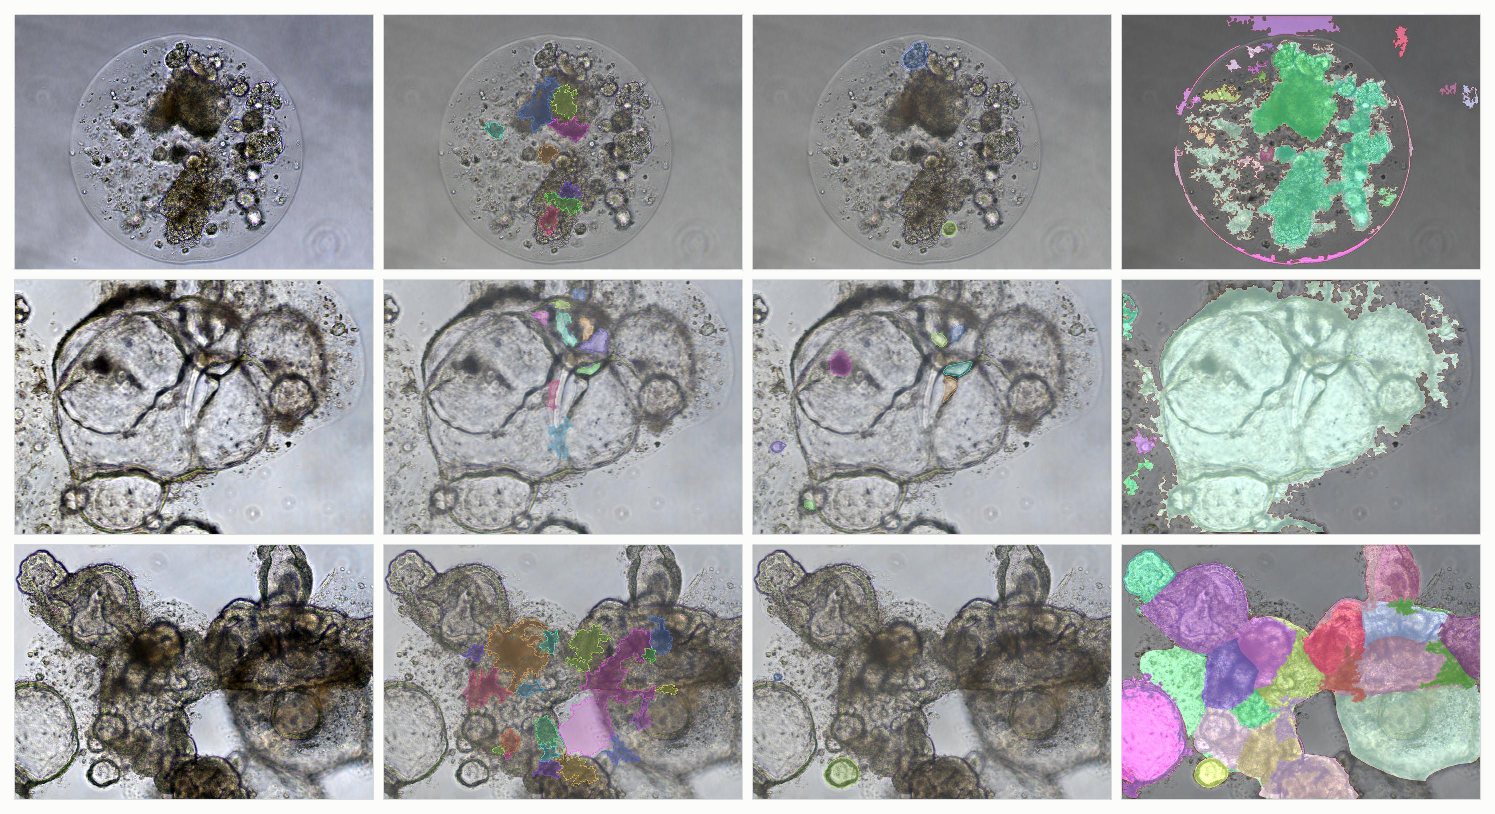
\includegraphics[width=\textwidth]{segmentation_method_comparison_app80_no_text.pdf}
\caption{\textbf{App80 Y-27632 segmentation comparison.}
Rows show representative 10~uM Y-27632 fields from 5, 10, and 12 December
2025, respectively. Columns show, from left to right: the raw brightfield image,
the early prompted-watershed overlay, the early CPSAM/SAM-style proposal overlay,
and the final AAPS multiscale large-object recovery overlay. The comparison
illustrates why a plain edge- or prompt-driven proposal was insufficient for the
App80 recovery experiment: organoid size and contrast changed over time, and
large or weakly bounded structures required a multiscale branch rather than a
single local-threshold or proposal method.}
\end{figure}

\begin{figure}[p]
\centering
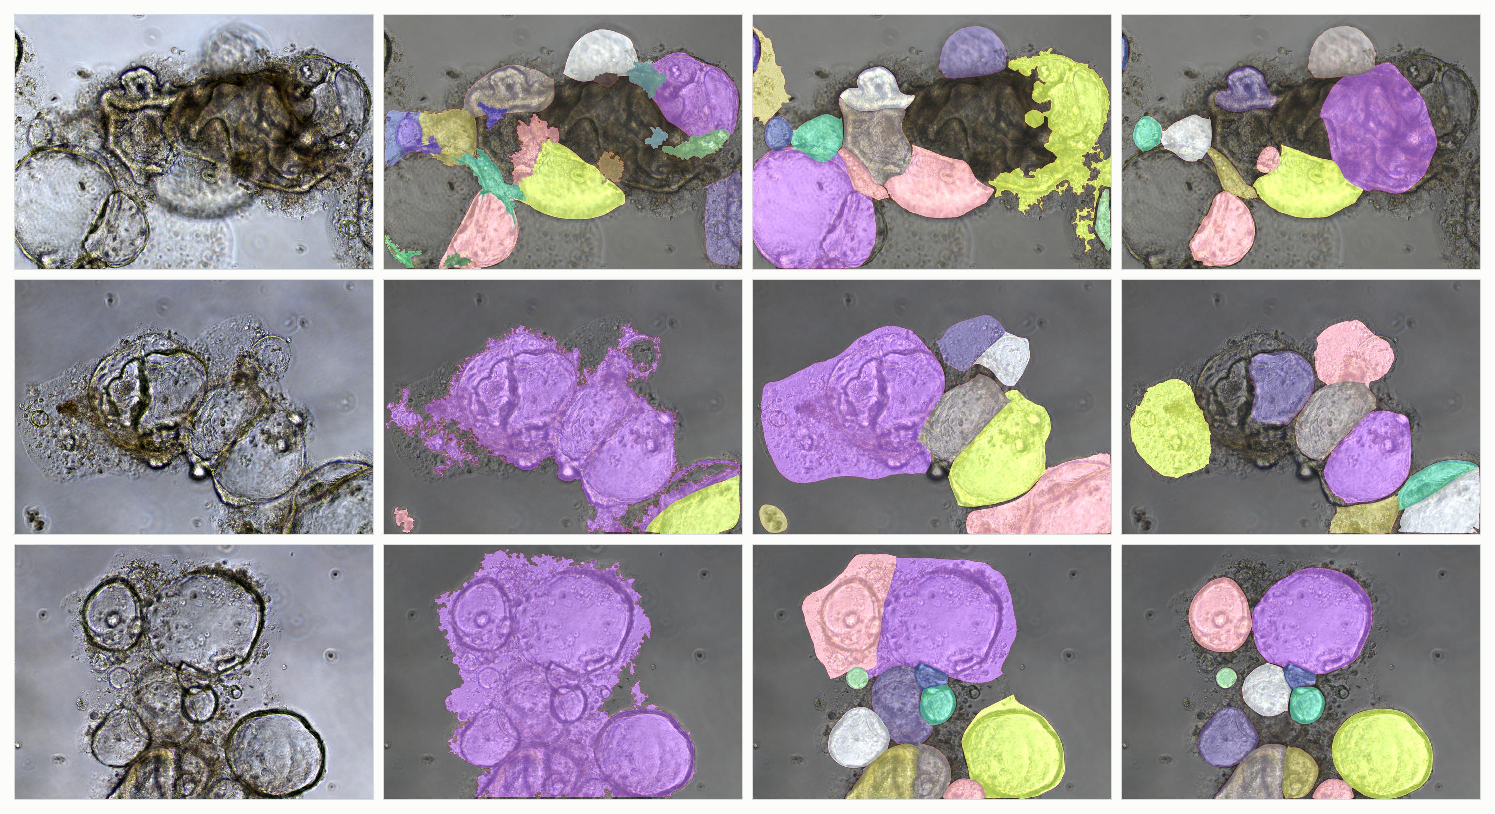
\includegraphics[width=\textwidth]{segmentation_method_comparison_app65_no_text.pdf}
\caption{\textbf{App65 alginate segmentation comparison.}
Rows show representative 0.02\% alginate fields from 29 November 2025
(10x00, 10x14, and 10x15). Columns show, from left to right: the raw
brightfield image, an older multiscale Cellpose large-recovery overlay, a
threshold-hinted Cellpose test overlay, and the final AAPS direct-brightfield
segmentation overlay. The comparison emphasizes that alginate-induced morphology
requires a branch that follows the actual brightfield organoid wall and internal
contrast, rather than over-weighting generic threshold evidence or a single
diameter prior.}
\end{figure}

\begin{figure}[p]
\centering
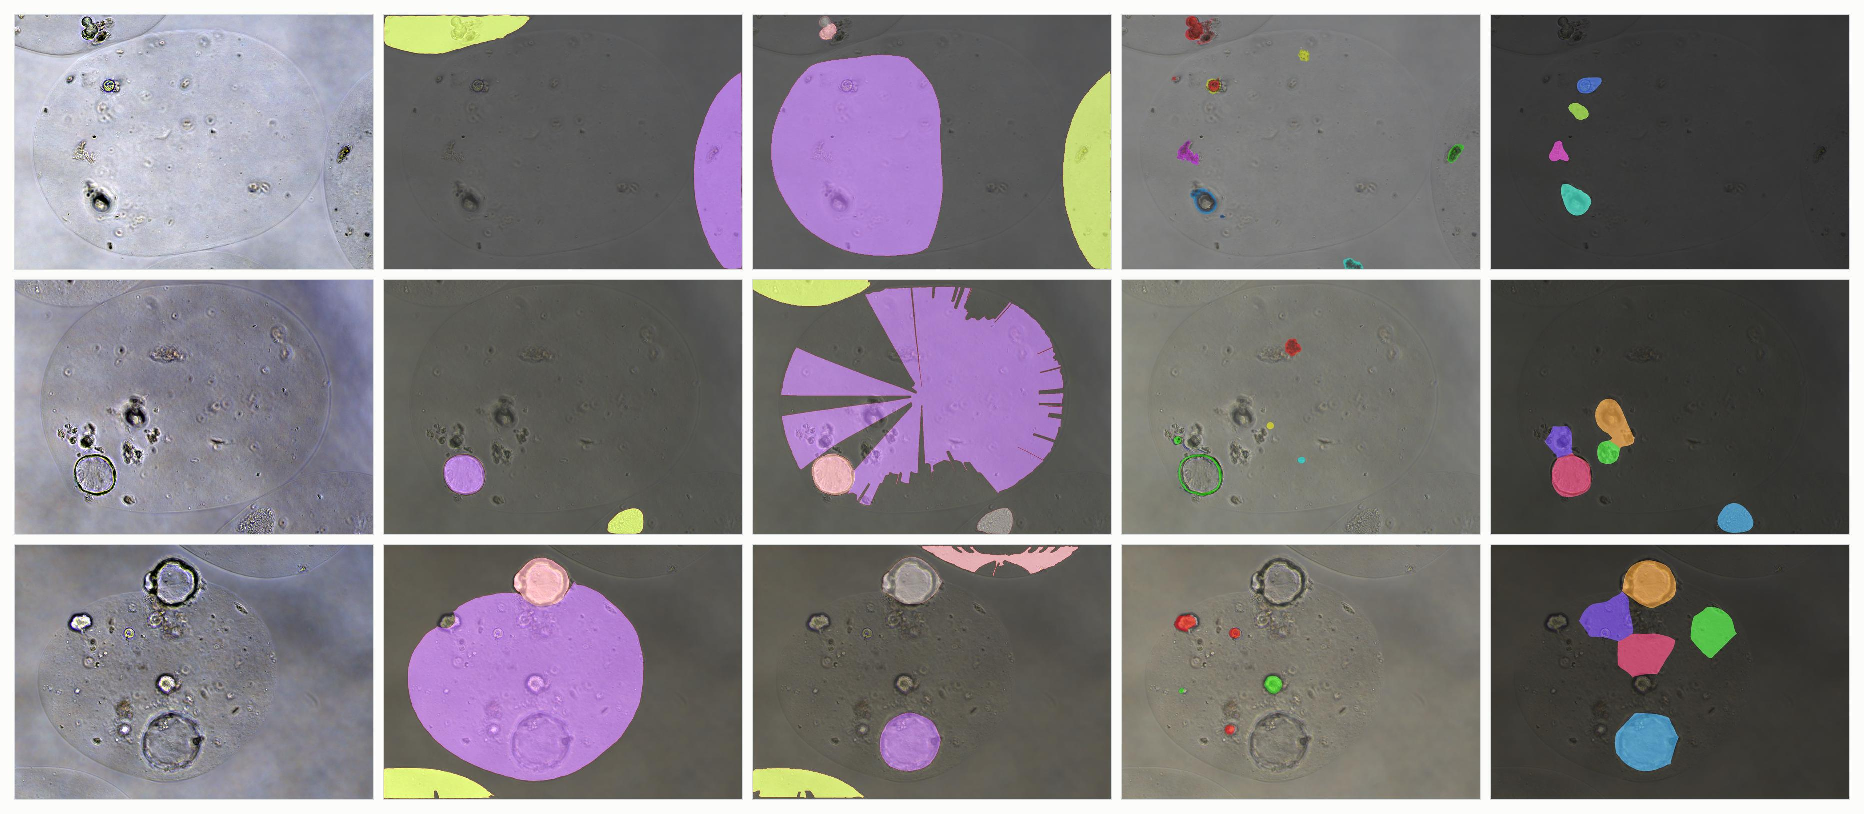
\includegraphics[width=\textwidth]{segmentation_method_comparison_app81_no_text.pdf}
\caption{\textbf{App81 density segmentation and image-generation-assisted
method routing.}
Rows show low-density App81 examples from 14, 15, and 16 October 2025,
respectively. Columns show, from left to right: the raw brightfield image,
threshold-hinted Cellpose, resized multiscale Cellpose, the image-generation
masking result, and the final stitched AAPS-selected hybrid overlay. The figure
summarizes the main App81 lesson: threshold and Cellpose variants are efficient
and reproducible for many panels, while image generation is useful as a targeted
semantic prior for cystic organoids. However, image-generation outputs must be
harnessed by panel-level QC and instance cleanup because they may merge adjacent
organoids or confuse a pale hydrogel boundary with an organoid.}
\end{figure}

\section*{Manuscript Interpretation}

These comparisons support the manuscript claim that the AAPS harness does not
depend on one universal segmentation algorithm. Instead, it records dataset
context, tests candidate segmentation branches, preserves intermediate outputs,
and routes each biological experiment to the method that best supports the
downstream measurement. This is important for organoid assays because growth,
differentiation, and fusion are not all optimized by the same mask behavior:
growth metrics favor robust area recovery, differentiation metrics depend on
darkness or wall-intensity stability, and fusion metrics require clean instance
boundaries and spatial structure.

The final figures should be cited as method-comparison evidence, not as a
standalone quantitative benchmark. They demonstrate visually why the final
App80, App65, and App81 pipelines were selected and why difficult panels were
handled by AAPS-style quality control and human-in-the-loop refinement rather
than by unguarded autonomous segmentation.

\end{document}
